\section{Vectors in Cartesian Space}

In the previous chapter, points of the plane were described by Cartesian
coordinates. We now use that numerical description to construct vectors. The
order is important: we begin with points and the arithmetic already available
for their coordinates, then introduce an arrow determined by an ordered pair of
points, decide geometrically when two such arrows are equal, and only then pass
to free vectors and operations on them.

The coordinate formulas will not replace the geometry. They will provide
practical criteria for recognising and calculating the geometric objects that
have already been introduced.

\subsection{Position Vectors and Displacement Vectors}

Let the origin of the coordinate system be $O=(0,0)$, and let
\[
A=(x_1,y_1),
\qquad
B=(x_2,y_2).
\]

The arrow from the origin to a point records the position of that point relative
to the chosen origin. We write
\[
\boxed{\mathbf r_A=\overrightarrow{OA}=(x_1,y_1)},
\qquad
\boxed{\mathbf r_B=\overrightarrow{OB}=(x_2,y_2)}.
\]
These are the \emph{position vectors} of $A$ and $B$.

If an object moves from $A$ to $B$, we are no longer asking where either point
is. We are asking what change carries the initial position to the final one. The
answer is the \emph{displacement vector}
\[
\Delta\mathbf r=\overrightarrow{AB}.
\]
Its components are obtained by subtracting the initial coordinates from the
final coordinates:
\[
\boxed{
\overrightarrow{AB}
=(x_2-x_1,\,y_2-y_1)
}.
\]

The relation between the two kinds of vectors is therefore
\[
\boxed{
\Delta\mathbf r
=\overrightarrow{AB}
=\mathbf r_B-\mathbf r_A
}.
\]
Equivalently,
\[
\boxed{
\mathbf r_B=\mathbf r_A+\Delta\mathbf r
}.
\]
The final position is obtained by adding the displacement to the initial
position.

\begin{center}
\begin{tikzpicture}[scale=0.9]
    \draw[axis] (-0.5,0) -- (7.0,0) node[right] {$x$};
    \draw[axis] (0,-0.5) -- (0,5.2) node[above] {$y$};

    \coordinate (O) at (0,0);
    \coordinate (A) at (2,1.4);
    \coordinate (B) at (5.4,4.0);

    \draw[helper,->] (O) -- (A)
        node[midway,below right] {$\mathbf r_A$};
    \draw[helper,->] (O) -- (B)
        node[midway,above left] {$\mathbf r_B$};
    \draw[subset,->] (A) -- (B)
        node[midway,below right] {$\Delta\mathbf r=\overrightarrow{AB}$};

    \fill (O) circle (2pt) node[below left] {$O$};
    \fill[geometricSubsetColor] (A) circle (2pt) node[below right] {$A$};
    \fill[geometricSubsetColor] (B) circle (2pt) node[above right] {$B$};
\end{tikzpicture}
\end{center}

A position vector depends on the chosen origin: moving the origin changes the
coordinates assigned to the same point. A displacement vector compares two
positions. If the whole coordinate system is translated, both position vectors
change in the same way, but their difference remains the same.

The same vector can also be drawn from another starting point. If
$P=(p_1,p_2)$ and
\[
\mathbf v=(v_1,v_2),
\]
then applying this displacement at $P$ produces
\[
Q=P+\mathbf v=(p_1+v_1,\,p_2+v_2).
\]
Thus a displacement vector is not tied to one particular place: it describes
the same change wherever it is applied.

The zero vector
\[
\boxed{\mathbf 0=(0,0)}
\]
means no displacement. The opposite vector
\[
\boxed{-\mathbf v=(-v_1,-v_2)}
\]
reverses a displacement. In particular,
\[
\boxed{\overrightarrow{BA}=-\overrightarrow{AB}}.
\]

For motion depending on time, the position will later be written as
$\mathbf r(t)$. The displacement between two moments $t_1$ and $t_2$ will then
have exactly the same form:
\[
\Delta\mathbf r
=\mathbf r(t_2)-\mathbf r(t_1).
\]

\subsection{Two Journeys Become One: Why Vectors Add}

Suppose a point is moved twice. The first displacement is
\[
\mathbf u=(u_1,u_2),
\]
and the second is
\[
\mathbf v=(v_1,v_2).
\]
We want one vector that has exactly the same final effect as these two moves
performed successively.

\begin{corebox}[The geometric problem]
Vector addition must represent the single displacement whose effect is identical
to performing two given displacements one after the other.
\end{corebox}

\begin{derivationbox}[Coordinate form forced by successive motion]
Start at an arbitrary point $(x,y)$. After applying $\mathbf u$ we are at
\[
(x+u_1,\,y+u_2).
\]
Applying $\mathbf v$ from there gives
\[
(x+u_1+v_1,\,y+u_2+v_2).
\]
Relative to the original point, the total horizontal change is $u_1+v_1$ and
the total vertical change is $u_2+v_2$. Therefore the coordinate rule is forced
by the meaning of successive displacement.
\end{derivationbox}

\begin{definitionbox}
For vectors $\mathbf u=(u_1,u_2)$ and $\mathbf v=(v_1,v_2)$, their sum is
\[
\boxed{
\mathbf u+\mathbf v
=
(u_1+v_1,\,u_2+v_2)
}.
\]
\end{definitionbox}

\begin{interpretationbox}[What coordinatewise addition records]
The formula is bookkeeping for a journey performed in two stages. It adds
changes of the same kind: horizontal change to horizontal change and vertical
change to vertical change.
\end{interpretationbox}

\begin{center}
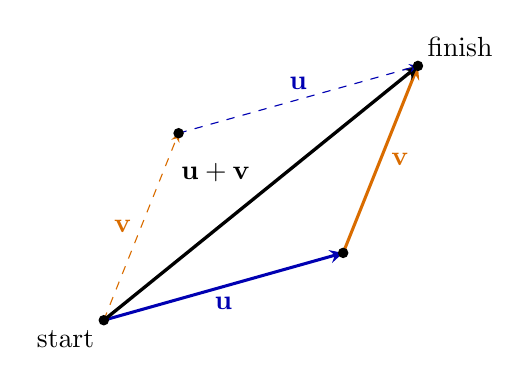
\begin{tikzpicture}[scale=0.95,>=stealth]
    \coordinate (O) at (0,0);
    \coordinate (U) at (3.2,0.9);
    \coordinate (V) at (1.0,2.5);
    \coordinate (S) at (4.2,3.4);

    \draw[blue!70!black,line width=1.1pt,->] (O) -- (U)
        node[midway,below] {$\mathbf u$};
    \draw[orange!85!black,line width=1.1pt,->] (U) -- (S)
        node[midway,right] {$\mathbf v$};
    \draw[very thick,->] (O) -- (S)
        node[midway,above left] {$\mathbf u+\mathbf v$};

    \draw[orange!85!black,dashed,->] (O) -- (V)
        node[midway,left] {$\mathbf v$};
    \draw[blue!70!black,dashed,->] (V) -- (S)
        node[midway,above] {$\mathbf u$};

    \fill (O) circle (2pt) node[below left] {start};
    \fill (U) circle (2pt);
    \fill (V) circle (2pt);
    \fill (S) circle (2pt) node[above right] {finish};
\end{tikzpicture}
\end{center}

\begin{proofbox}[Why the order does not change the result]
The diagram contains two routes to the same endpoint:
\[
\mathbf u\text{ then }\mathbf v,
\qquad
\mathbf v\text{ then }\mathbf u.
\]
They agree because addition of real numbers is commutative:
\[
u_1+v_1=v_1+u_1,
\qquad
u_2+v_2=v_2+u_2.
\]
Therefore
\[
\mathbf u+\mathbf v=\mathbf v+\mathbf u.
\]
\end{proofbox}

\begin{theorembox}
Vector addition is commutative:
\[
\boxed{\mathbf u+\mathbf v=\mathbf v+\mathbf u}.
\]
Geometrically, this is the parallelogram rule.
\end{theorembox}

Subtraction answers a different practical question: what displacement must be
performed after $\mathbf v$ in order to have the same effect as $\mathbf u$?
We seek a vector $\mathbf w$ satisfying
\[
\mathbf v+\mathbf w=\mathbf u.
\]

\begin{derivationbox}[Subtraction as the missing displacement]
Solving the equation $\mathbf v+\mathbf w=\mathbf u$ coordinate by coordinate
gives
\[
\mathbf w=(u_1-v_1,\,u_2-v_2).
\]
\end{derivationbox}

\begin{definitionbox}
For vectors $\mathbf u=(u_1,u_2)$ and $\mathbf v=(v_1,v_2)$,
\[
\boxed{
\mathbf u-\mathbf v
=
(u_1-v_1,\,u_2-v_2)
}.
\]
In particular,
\[
\boxed{\overrightarrow{AB}=B-A}.
\]
\end{definitionbox}

\begin{remarkbox}
The expression $B-A$ does not subtract geometric points as physical objects. It
subtracts their coordinate addresses to recover the displacement carrying one
point to the other.
\end{remarkbox}

\subsection{Repeating and Reversing a Displacement}

Repeating $\mathbf v=(v_1,v_2)$ twice gives $(2v_1,2v_2)$, while reversing it
gives $(-v_1,-v_2)$. The natural extension is
\[
\lambda\mathbf v=(\lambda v_1,\lambda v_2),
\qquad \lambda\in\mathbb R.
\]
For positive $\lambda$ the orientation is unchanged; for negative $\lambda$ it
is reversed.

\subsection{Linear Combinations: What Addition and Scaling Can Build}

Addition and scalar multiplication were introduced as two separate operations,
but they are most useful when they are combined. Given vectors $\mathbf u$ and
$\mathbf v$ and real numbers $a$ and $b$, the vector
\[
a\mathbf u+b\mathbf v
\]
is called a \emph{linear combination} of $\mathbf u$ and $\mathbf v$.

The phrase has a direct geometric meaning. First scale $\mathbf u$ by $a$ and
$\mathbf v$ by $b$; then add the two resulting displacements. Thus a linear
combination is not a new operation. It is a controlled use of the two operations
already understood.

\begin{center}
\begin{tikzpicture}[scale=0.9,>=stealth]
    \coordinate (O) at (0,0);
    \coordinate (AU) at (3.4,0.9);
    \coordinate (BV) at (1.0,2.7);
    \coordinate (S) at (4.4,3.6);

    \draw[blue!70!black,line width=1.1pt,->] (O) -- (AU)
        node[midway,below] {$a\mathbf u$};
    \draw[orange!85!black,line width=1.1pt,->] (AU) -- (S)
        node[midway,right] {$b\mathbf v$};
    \draw[very thick,->] (O) -- (S)
        node[midway,above left] {$a\mathbf u+b\mathbf v$};
    \draw[helper,dashed] (O) -- (BV);
    \draw[helper,dashed] (BV) -- (S);
\end{tikzpicture}
\end{center}

A single nonzero vector can generate only one line through the origin:
\[
\{\lambda\mathbf v:\lambda\in\mathbb R\}.
\]
Changing $\lambda$ changes the length and possibly the orientation, but never
the underlying line of motion.

Two vectors behave differently. If $\mathbf u$ and $\mathbf v$ are parallel,
then every linear combination still lies on one line. If they are not parallel,
then their linear combinations fill the whole plane. Geometrically, the two
independent directions allow us to reach any endpoint by a suitable
parallelogram.

\begin{theorembox}
Two nonparallel vectors $\mathbf u$ and $\mathbf v$ determine every vector in
the plane uniquely in the form
\[
\mathbf w=a\mathbf u+b\mathbf v.
\]
The numbers $a$ and $b$ record how much motion occurs in each chosen direction.
\end{theorembox}

This observation is the bridge to the later notion of a basis. A basis is not
an unrelated new object: it is a pair of directions whose linear combinations
can describe every vector uniquely.
\subsection{How Much Motion and in Which Direction?}

The coordinate pair of a vector records two changes, but it does not immediately
answer two basic geometric questions.

\begin{corebox}[Two questions carried by every nonzero vector]
\begin{enumerate}
    \item How long is the displacement?
    \item In which direction does it point?
\end{enumerate}
\end{corebox}

Let
\[
\mathbf v=(v_1,v_2)
\]
be drawn from the origin. Its endpoint, together with its horizontal and
vertical coordinate changes, forms a right triangle. The legs have lengths
$|v_1|$ and $|v_2|$, while the vector itself is the hypotenuse.

\begin{center}
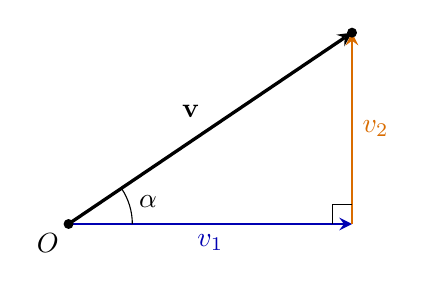
\begin{tikzpicture}[scale=0.9,>=stealth]
    \coordinate (O) at (0,0);
    \coordinate (P) at (4,2.7);
    \coordinate (R) at (4,0);

    \draw[very thick,->] (O) -- (P)
        node[midway,above left] {$\mathbf v$};
    \draw[blue!70!black,line width=1pt,->] (O) -- (R)
        node[midway,below] {$v_1$};
    \draw[orange!85!black,line width=1pt,->] (R) -- (P)
        node[midway,right] {$v_2$};
    \draw (R) ++(-0.28,0) -- ++(0,0.28) -- ++(0.28,0);

    \draw (0.9,0) arc[start angle=0,end angle=34.0,radius=0.9];
    \node at (1.12,0.32) {$\alpha$};
    \fill (O) circle (2pt) node[below left] {$O$};
    \fill (P) circle (2pt);
\end{tikzpicture}
\end{center}

\begin{derivationbox}[Length from the Pythagorean theorem]
The right triangle gives
\[
\|\mathbf v\|^2=v_1^2+v_2^2.
\]
The length is nonnegative, so
\[
\|\mathbf v\|=\sqrt{v_1^2+v_2^2}.
\]
\end{derivationbox}

\begin{definitionbox}
The Euclidean length, or norm, of $\mathbf v=(v_1,v_2)$ is
\[
\boxed{\|\mathbf v\|=\sqrt{v_1^2+v_2^2}}.
\]
The double bars distinguish the vector from the number measuring its length.
\end{definitionbox}

\begin{theorembox}
\[
\boxed{\|\mathbf0\|=0},
\qquad
\boxed{\mathbf v\neq\mathbf0\implies\|\mathbf v\|>0}.
\]
Moreover, for points $A$ and $B$,
\[
\boxed{d_E(A,B)=\|B-A\|}.
\]
\end{theorembox}

\begin{interpretationbox}[A displacement packages distance and direction]
The vector $B-A$ records how to move from $A$ to $B$, while its norm records the
Euclidean distance travelled. The same object therefore carries both directional
and metric information.
\end{interpretationbox}

Now assume $\mathbf v\neq\mathbf0$ and let $\alpha$ be its angle of inclination,
measured from the positive $x$-axis.

\begin{derivationbox}[Separating magnitude from direction]
The right triangle gives
\[
\cos\alpha=\frac{v_1}{\|\mathbf v\|},
\qquad
\sin\alpha=\frac{v_2}{\|\mathbf v\|}.
\]
Therefore
\[
v_1=\|\mathbf v\|\cos\alpha,
\qquad
v_2=\|\mathbf v\|\sin\alpha.
\]
\end{derivationbox}

\begin{theorembox}
Every nonzero vector admits the decomposition
\[
\boxed{
\mathbf v=\|\mathbf v\|(\cos\alpha,\sin\alpha)
}.
\]
The vector $(\cos\alpha,\sin\alpha)$ has length one.
\end{theorembox}

\begin{interpretationbox}[The two pieces of a vector]
\begin{itemize}
    \item $\|\mathbf v\|$ says how much displacement occurs;
    \item $(\cos\alpha,\sin\alpha)$ says in which direction it occurs.
\end{itemize}
Thus every nonzero vector is a positive magnitude multiplied by a unit direction.
\end{interpretationbox}

\subsection{One Angle Calculation, Two Geometric Tests}

Take two arbitrary nonzero vectors
\[
\mathbf u=(u_1,u_2),
\qquad
\mathbf v=(v_1,v_2).
\]
Let their angles of inclination be $\alpha$ and $\beta$. Then
\[
\mathbf u=\|\mathbf u\|(\cos\alpha,\sin\alpha),
\qquad
\mathbf v=\|\mathbf v\|(\cos\beta,\sin\beta).
\]

\begin{corebox}[One comparison controls both tests]
The directed turn from $\mathbf u$ to $\mathbf v$ is $\beta-\alpha$. Its sine
detects parallel directions, while its cosine detects perpendicular directions.
The coordinate tests will be derived from these geometric facts.
\end{corebox}

\begin{center}
\begin{tikzpicture}[scale=0.9]
    \coordinate (O) at (0,0);
    \coordinate (U) at (4.2,1.6);
    \coordinate (V) at (1.6,3.6);
    \draw[axis] (-0.4,0) -- (5.2,0) node[right] {$x$};
    \draw[subset,->] (O) -- (U) node[above right] {$\mathbf u$};
    \draw[subset,->] (O) -- (V) node[above] {$\mathbf v$};
    \draw (0.8,0) arc[start angle=0,end angle=20.9,radius=0.8];
    \node at (0.97,0.18) {$\alpha$};
    \draw (0.66,0.25) arc[start angle=20.9,end angle=66.0,radius=0.71];
    \node at (0.61,0.62) {$\theta$};
    \draw (1.35,0) arc[start angle=0,end angle=66.0,radius=1.35];
    \node at (1.02,1.08) {$\beta$};
\end{tikzpicture}
\end{center}

\subsubsection{Parallel directions arise from the sine of the angle difference}

\begin{derivationbox}[Deriving the determinant test]
Two nonzero vectors determine the same unoriented direction precisely when
\[
\beta-\alpha\equiv0\pmod{\pi},
\]
equivalently when $\sin(\beta-\alpha)=0$. Using
\[
\sin(\beta-\alpha)=\sin\beta\cos\alpha-\cos\beta\sin\alpha
\]
and substituting
\[
\cos\alpha=\frac{u_1}{\|\mathbf u\|},
\quad
\sin\alpha=\frac{u_2}{\|\mathbf u\|},
\quad
\cos\beta=\frac{v_1}{\|\mathbf v\|},
\quad
\sin\beta=\frac{v_2}{\|\mathbf v\|},
\]
we obtain
\[
\sin(\beta-\alpha)
=
\frac{u_1v_2-u_2v_1}{\|\mathbf u\|\,\|\mathbf v\|}.
\]
The denominator is nonzero, so the sine vanishes exactly when the numerator
vanishes.
\end{derivationbox}

\begin{theorembox}
For nonzero vectors in the plane,
\[
\boxed{
\mathbf u\parallel\mathbf v
\iff
u_1v_2-u_2v_1=0
}.
\]
Equivalently,
\[
\boxed{
\mathbf u\parallel\mathbf v
\iff
\mathbf u=\lambda\mathbf v
\text{ for some }\lambda\neq0
}.
\]
\end{theorembox}

\begin{proofbox}[Why the determinant condition gives a scalar multiple]
If $v_1\neq0$, set $\lambda=u_1/v_1$. The equality
$u_1v_2-u_2v_1=0$ gives $u_2=\lambda v_2$, hence
$\mathbf u=\lambda\mathbf v$. If $v_1=0$, then $v_2\neq0$ and the same argument
uses $\lambda=u_2/v_2$.
\end{proofbox}

\begin{interpretationbox}[Meaning of the determinant expression]
The quantity $u_1v_2-u_2v_1$ measures whether the two coordinate directions
span genuine area. It is zero exactly when both vectors lie on one line.
\end{interpretationbox}

\subsubsection{The cosine of the same difference reveals perpendicularity}

\begin{derivationbox}[Deriving the dot-product test]
The vectors are perpendicular precisely when
\[
\beta-\alpha\equiv\frac{\pi}{2}\pmod{\pi},
\]
equivalently when $\cos(\beta-\alpha)=0$. The identity
\[
\cos(\beta-\alpha)
=
\cos\beta\cos\alpha+\sin\beta\sin\alpha
\]
gives
\[
\cos(\beta-\alpha)
=
\frac{u_1v_1+u_2v_2}{\|\mathbf u\|\,\|\mathbf v\|}.
\]
Since the denominator is nonzero, perpendicularity is equivalent to the
vanishing of the numerator.
\end{derivationbox}

\begin{definitionbox}
For vectors in the plane, the \emph{dot product} is
\[
\boxed{
\mathbf u\cdot\mathbf v=u_1v_1+u_2v_2
}.
\]
In three-dimensional space,
\[
\boxed{
(u_1,u_2,u_3)\cdot(v_1,v_2,v_3)
=u_1v_1+u_2v_2+u_3v_3
}.
\]
\end{definitionbox}

\begin{theorembox}
For nonzero vectors,
\[
\boxed{
\mathbf u\perp\mathbf v
\iff
\mathbf u\cdot\mathbf v=0
}.
\]
More generally, if $\theta$ is the smaller angle between them, then
\[
\boxed{
\mathbf u\cdot\mathbf v
=
\|\mathbf u\|\,\|\mathbf v\|\cos\theta
}.
\]
\end{theorembox}

\begin{interpretationbox}[What the sign of the dot product says]
The dot product is positive for an acute angle, zero for a right angle, and
negative for an obtuse angle. It converts angular information into one scalar.
\end{interpretationbox}

\begin{examplebox}
Take
\[
\mathbf u=(3,2),
\qquad
\mathbf v=(-2,3).
\]
Then
\[
\mathbf u\cdot\mathbf v=3(-2)+2(3)=0.
\]
Therefore $\cos\theta=0$, so the vectors are perpendicular.
\end{examplebox}

\begin{summarybox}[Two coordinate tests from one geometric comparison]
The sine of the angle difference produces the parallelism test
$u_1v_2-u_2v_1=0$. The cosine of the same difference produces the
perpendicularity test $\mathbf u\cdot\mathbf v=0$. Neither rule is imposed
arbitrarily; both are consequences of the geometry of angle.
\end{summarybox}

\subsection{Why the Dot Product Can Be Expanded}

The dot product was discovered from the cosine of the angle between two
vectors. Before using it in longer calculations, we must verify how it behaves
under addition and scalar multiplication.

Let
\[
\mathbf u=(u_1,u_2),\qquad
\mathbf v=(v_1,v_2),\qquad
\mathbf w=(w_1,w_2).
\]
Then
\[
\begin{aligned}
(\mathbf u+\mathbf w)\cdot\mathbf v
&=(u_1+w_1)v_1+(u_2+w_2)v_2\\
&=(u_1v_1+u_2v_2)+(w_1v_1+w_2v_2)\\
&=\mathbf u\cdot\mathbf v+\mathbf w\cdot\mathbf v.
\end{aligned}
\]
Thus the dot product distributes over vector addition. Similarly,
\[
(\lambda\mathbf u)\cdot\mathbf v
=\lambda(\mathbf u\cdot\mathbf v).
\]
The symmetry of multiplication of real numbers also gives
\[
\mathbf u\cdot\mathbf v=\mathbf v\cdot\mathbf u.
\]

\begin{theorembox}
For vectors $\mathbf u,\mathbf v,\mathbf w$ and a real number $\lambda$,
\[
\begin{aligned}
(\mathbf u+\mathbf w)\cdot\mathbf v
&=\mathbf u\cdot\mathbf v+\mathbf w\cdot\mathbf v,\\
(\lambda\mathbf u)\cdot\mathbf v
&=\lambda(\mathbf u\cdot\mathbf v),\\
\mathbf u\cdot\mathbf v
&=\mathbf v\cdot\mathbf u.
\end{aligned}
\]
Moreover,
\[
\boxed{\mathbf u\cdot\mathbf u=\|\mathbf u\|^2}.
\]
\end{theorembox}

The last identity follows immediately:
\[
\mathbf u\cdot\mathbf u=u_1^2+u_2^2=\|\mathbf u\|^2.
\]
These properties justify every later expansion involving expressions such as
$(\mathbf u-\mathbf v)\cdot(\mathbf u-\mathbf v)$. They are not formal rules
borrowed from elsewhere; they follow from the coordinate definition of the dot
product.
\subsection{The Angle Between Two Vectors}

The difference of inclination angles $\beta-\alpha$ is a directed turn and is
understood modulo a full turn. The ordinary angle between two nonzero vectors is
a different object: it is the smaller, unoriented separation between their
directions.

\begin{definitionbox}
For nonzero vectors $\mathbf u$ and $\mathbf v$, their angle is the unique number
\[
\theta\in[0,\pi]
\]
satisfying
\[
\boxed{
\cos\theta
=
\frac{\mathbf u\cdot\mathbf v}
{\|\mathbf u\|\,\|\mathbf v\|}
}.
\]
\end{definitionbox}

The interval $[0,\pi]$ chooses the smaller unoriented angle. Thus directions
with inclinations $10^\circ$ and $350^\circ$ are separated by $20^\circ$, not
$340^\circ$.

The definition agrees with the earlier geometric interpretation:
\[
\theta=0 \iff \text{same direction},
\qquad
\theta=\frac{\pi}{2} \iff \text{perpendicular},
\qquad
\theta=\pi \iff \text{opposite directions}.
\]
The Cauchy--Schwarz inequality proved later guarantees that the quotient inside
the cosine lies between $-1$ and $1$.
\subsection{The Cosine Theorem Emerges Immediately}

Draw $\mathbf u$ and $\mathbf v$ from a common point. The displacement from the
endpoint of $\mathbf v$ to the endpoint of $\mathbf u$ is
\[
\mathbf u-\mathbf v.
\]
Thus these three vectors determine a triangle with side lengths
\[
\|\mathbf u\|,
\qquad
\|\mathbf v\|,
\qquad
\|\mathbf u-\mathbf v\|.
\]

\begin{derivationbox}[Expanding the third side]
\[
\begin{aligned}
\|\mathbf u-\mathbf v\|^2
&=(\mathbf u-\mathbf v)\cdot(\mathbf u-\mathbf v)\\
&=\mathbf u\cdot\mathbf u
-\mathbf u\cdot\mathbf v
-\mathbf v\cdot\mathbf u
+\mathbf v\cdot\mathbf v\\
&=\|\mathbf u\|^2+\|\mathbf v\|^2-2\mathbf u\cdot\mathbf v\\
&=\|\mathbf u\|^2+\|\mathbf v\|^2
-2\|\mathbf u\|\,\|\mathbf v\|\cos\theta.
\end{aligned}
\]
If
\[
a=\|\mathbf u\|,
\qquad
b=\|\mathbf v\|,
\qquad
c=\|\mathbf u-\mathbf v\|,
\]
then the familiar triangle formula follows.
\end{derivationbox}

\begin{theorembox}
For a triangle with side lengths $a$, $b$, and $c$, where $\theta$ is the angle
between the sides of lengths $a$ and $b$,
\[
\boxed{c^2=a^2+b^2-2ab\cos\theta}.
\]
\end{theorembox}

\begin{interpretationbox}[Why the theorem appears here]
The cosine theorem is not inserted as an external formula. It is the expansion
of the squared displacement between the endpoints of two arbitrary vectors.
The triangle law is therefore encoded in vector subtraction and the dot product.
\end{interpretationbox}

\begin{center}
\begin{tikzpicture}[scale=0.9]
    \coordinate (O) at (0,0);
    \coordinate (U) at (4.4,1.5);
    \coordinate (V) at (1.3,3.5);
    \draw[subset,->] (O) -- (U) node[midway,below] {$\mathbf u$};
    \draw[subset,->] (O) -- (V) node[midway,left] {$\mathbf v$};
    \draw[very thick,->] (V) -- (U) node[midway,above right] {$\mathbf u-\mathbf v$};
    \draw (0.72,0.25) arc[start angle=19,end angle=69.6,radius=0.76];
    \node at (0.70,0.65) {$\theta$};
\end{tikzpicture}
\end{center}

\subsection{Projection Is Forced by the Right-Angle Condition}

Let $\mathbf v\neq\mathbf0$. We seek a multiple $\lambda\mathbf v$ such that
the remainder
\[
\mathbf u-\lambda\mathbf v
\]
is perpendicular to $\mathbf v$. The criterion just derived requires
\[
(\mathbf u-\lambda\mathbf v)\cdot\mathbf v=0.
\]
Expanding gives
\[
\mathbf u\cdot\mathbf v-
\lambda(\mathbf v\cdot\mathbf v)=0,
\]
so
\[
\lambda
=
\frac{\mathbf u\cdot\mathbf v}{\mathbf v\cdot\mathbf v}.
\]
Thus the parallel component is
\[
\operatorname{proj}_{\mathbf v}\mathbf u
=
\frac{\mathbf u\cdot\mathbf v}{\mathbf v\cdot\mathbf v}\,\mathbf v.
\]
The formula is the solution of a geometric requirement, not a rule to be
memorised without explanation.

\subsection{Orthogonal Decomposition and Its Consequences}

The projection formula splits $\mathbf u$ into two geometrically different parts:
\[
\mathbf u
=
\operatorname{proj}_{\mathbf v}\mathbf u
+
\left(\mathbf u-\operatorname{proj}_{\mathbf v}\mathbf u\right).
\]
The first term is parallel to $\mathbf v$ and the second is perpendicular to
$\mathbf v$. This is the orthogonal decomposition of $\mathbf u$ relative to
the direction of $\mathbf v$.

Because the two components are perpendicular, the Pythagorean theorem gives
\[
\boxed{
\|\mathbf u\|^2
=
\left\|\operatorname{proj}_{\mathbf v}\mathbf u\right\|^2
+
\left\|\mathbf u-\operatorname{proj}_{\mathbf v}\mathbf u\right\|^2
}.
\]

\subsubsection*{Scalar component and vector projection}

The signed scalar component of $\mathbf u$ in the direction of nonzero
$\mathbf v$ is
\[
\boxed{
\operatorname{comp}_{\mathbf v}\mathbf u
=
\frac{\mathbf u\cdot\mathbf v}{\|\mathbf v\|}
}.
\]
It measures how much signed length of $\mathbf u$ lies along the direction of
$\mathbf v$. The vector projection is obtained by multiplying this number by
the unit vector in that direction:
\[
\operatorname{proj}_{\mathbf v}\mathbf u
=
\operatorname{comp}_{\mathbf v}\mathbf u
\frac{\mathbf v}{\|\mathbf v\|}.
\]

\subsubsection*{The Cauchy--Schwarz inequality}

The length of the parallel component cannot exceed the length of the entire
vector:
\[
\left|\operatorname{comp}_{\mathbf v}\mathbf u\right|
\leq \|\mathbf u\|.
\]
Substitution gives
\[
\boxed{
|\mathbf u\cdot\mathbf v|
\leq
\|\mathbf u\|\,\|\mathbf v\|
}.
\]
Therefore
\[
-1\leq
\frac{\mathbf u\cdot\mathbf v}
{\|\mathbf u\|\,\|\mathbf v\|}
\leq1,
\]
which guarantees that the angle formula using $\arccos$ is meaningful.

\subsubsection*{The triangle inequality}

The direct displacement $\mathbf u+\mathbf v$ cannot be longer than travelling
first by $\mathbf u$ and then by $\mathbf v$. Algebraically,
\[
\begin{aligned}
\|\mathbf u+\mathbf v\|^2
&=\|\mathbf u\|^2+2\mathbf u\cdot\mathbf v+\|\mathbf v\|^2\\
&\leq\|\mathbf u\|^2+2\|\mathbf u\|\,\|\mathbf v\|+\|\mathbf v\|^2\\
&=(\|\mathbf u\|+\|\mathbf v\|)^2.
\end{aligned}
\]
Hence
\[
\boxed{
\|\mathbf u+\mathbf v\|
\leq
\|\mathbf u\|+\|\mathbf v\|
}.
\]
This is the algebraic form of the geometric fact that the straight segment is
the shortest route between two points.
\subsection{From the Plane to Three-Dimensional Vectors}

Adding a third coordinate does not change the basic meaning of a vector. A
vector still records a displacement, but now it records three independent
coordinate changes:
\[
\mathbf v=(v_1,v_2,v_3).
\]
Addition and scalar multiplication remain componentwise, because successive
changes in each coordinate direction still combine independently.

Applying the Pythagorean theorem first to the first two coordinate changes and
then to the third gives
\[
\boxed{
\|\mathbf v\|
=
\sqrt{v_1^2+v_2^2+v_3^2}
}.
\]
The dot product extends in exactly the same way:
\[
\boxed{
\mathbf u\cdot\mathbf v
=
u_1v_1+u_2v_2+u_3v_3
}.
\]
Its geometric role is unchanged:
\[
\mathbf u\cdot\mathbf v
=
\|\mathbf u\|\,\|\mathbf v\|\cos\theta.
\]
Consequently,
\[
\boxed{
\mathbf u\perp\mathbf v
\iff
\mathbf u\cdot\mathbf v=0
}.
\]
Thus the dot product detects perpendicularity in both two and three dimensions.

\subsubsection*{A second product available in three dimensions}

In three dimensions there is another natural question. Given two vectors
\(\mathbf u\) and \(\mathbf v\), can we construct a new vector perpendicular to
both of them?

\begingroup
\setlength{\fboxsep}{9pt}

\begin{center}
\fcolorbox{blue!65!black}{blue!4}{%
\begin{minipage}{0.90\textwidth}
\textcolor{blue!65!black}{\textbf{Step 1: translate the geometric requirement into equations.}}

Let
\[
\mathbf u=(u_1,u_2,u_3),
\qquad
\mathbf v=(v_1,v_2,v_3),
\qquad
\mathbf n=(n_1,n_2,n_3).
\]
We require \(\mathbf n\) to be perpendicular to both inputs:
\[
\mathbf n\cdot\mathbf u=0,
\qquad
\mathbf n\cdot\mathbf v=0.
\]
Therefore
\[
\begin{aligned}
u_1n_1+u_2n_2+u_3n_3&=0,\\
v_1n_1+v_2n_2+v_3n_3&=0.
\end{aligned}
\]
\end{minipage}}
\end{center}

\begin{center}
\fcolorbox{violet!65!black}{violet!4}{%
\begin{minipage}{0.90\textwidth}
\textcolor{violet!65!black}{\textbf{Step 2: choose one component so that the remaining system is easy.}}

Set
\[
\textcolor{violet!75!black}{\Delta=u_1v_2-u_2v_1}.
\]
Assume first that \(\Delta\neq0\), and choose
\[
\textcolor{violet!75!black}{n_3=\Delta}.
\]
The two equations reduce to the ordinary \(2\times2\) system
\[
\begin{aligned}
u_1n_1+u_2n_2&=-u_3\Delta,\\
v_1n_1+v_2n_2&=-v_3\Delta.
\end{aligned}
\]
\end{minipage}}
\end{center}

\begin{center}
\fcolorbox{orange!80!black}{orange!5}{%
\begin{minipage}{0.90\textwidth}
\textcolor{orange!80!black}{\textbf{Step 3: eliminate \(n_2\) and find \(n_1\).}}

Multiply the first equation by \(v_2\), the second by \(u_2\), and subtract:
\[
\begin{aligned}
&v_2(u_1n_1+u_2n_2)
-u_2(v_1n_1+v_2n_2)\\
&\qquad=-u_3v_2\Delta+u_2v_3\Delta.
\end{aligned}
\]
The \(n_2\)-terms cancel, so
\[
\Delta n_1=\Delta(u_2v_3-u_3v_2).
\]
Since \(\Delta\neq0\),
\[
\boxed{\textcolor{orange!80!black}{n_1=u_2v_3-u_3v_2}}.
\]
\end{minipage}}
\end{center}

\begin{center}
\fcolorbox{orange!80!black}{orange!5}{%
\begin{minipage}{0.90\textwidth}
\textcolor{orange!80!black}{\textbf{Step 4: eliminate \(n_1\) and find \(n_2\).}}

Multiply the first equation by \(v_1\), the second by \(u_1\), and subtract:
\[
\begin{aligned}
&v_1(u_1n_1+u_2n_2)
-u_1(v_1n_1+v_2n_2)\\
&\qquad=-u_3v_1\Delta+u_1v_3\Delta.
\end{aligned}
\]
The \(n_1\)-terms cancel, giving
\[
-\Delta n_2=\Delta(u_1v_3-u_3v_1).
\]
Hence
\[
\boxed{\textcolor{orange!80!black}{n_2=u_3v_1-u_1v_3}}.
\]
\end{minipage}}
\end{center}

\begin{center}
\fcolorbox{green!55!black}{green!4}{%
\begin{minipage}{0.90\textwidth}
\textcolor{green!45!black}{\textbf{Step 5: assemble the three components.}}

Together with
\[
\textcolor{violet!75!black}{n_3=u_1v_2-u_2v_1},
\]
we obtain
\[
\boxed{
\mathbf n
=
\bigl(
\textcolor{orange!80!black}{u_2v_3-u_3v_2},
\;\textcolor{orange!80!black}{u_3v_1-u_1v_3},
\;\textcolor{violet!75!black}{u_1v_2-u_2v_1}
\bigr)
}.
\]
If the displayed \(\Delta\) is zero but the vectors are not parallel, one of the
other two coordinate pairs is nonzero. Repeating the same elimination with that
pair gives the same cyclic formula.
\end{minipage}}
\end{center}

\begin{center}
\fcolorbox{gray!70!black}{gray!5}{%
\begin{minipage}{0.90\textwidth}
\textcolor{gray!70!black}{\textbf{Step 6: verify that the constructed vector really works.}}

For the first input vector, the terms cancel in three visible pairs:
\[
\begin{aligned}
\mathbf n\cdot\mathbf u
&=\textcolor{blue!65!black}{(u_1u_2v_3-u_1u_2v_3)}\\
&\quad+\textcolor{orange!80!black}{(-u_1u_3v_2+u_1u_3v_2)}\\
&\quad+\textcolor{green!45!black}{(u_2u_3v_1-u_2u_3v_1)}\\
&=0.
\end{aligned}
\]
Likewise,
\[
\begin{aligned}
\mathbf n\cdot\mathbf v
&=\textcolor{blue!65!black}{(u_2v_1v_3-u_2v_1v_3)}\\
&\quad+\textcolor{orange!80!black}{(-u_3v_1v_2+u_3v_1v_2)}\\
&\quad+\textcolor{green!45!black}{(-u_1v_2v_3+u_1v_2v_3)}\\
&=0.
\end{aligned}
\]
Thus \(\mathbf n\perp\mathbf u\) and \(\mathbf n\perp\mathbf v\).
\end{minipage}}
\end{center}

\endgroup

The vector has therefore been derived from the two perpendicularity equations.
We now give it a name:
\[
\boxed{
\mathbf u\times\mathbf v
=
\bigl(
u_2v_3-u_3v_2,
\;u_3v_1-u_1v_3,
\;u_1v_2-u_2v_1
\bigr)
}.
\]
Consequently,
\[
\boxed{
(\mathbf u\times\mathbf v)\cdot\mathbf u=0,
\qquad
(\mathbf u\times\mathbf v)\cdot\mathbf v=0
}.
\]

The statement is stronger. Every linear combination
\[
a\mathbf u+b\mathbf v
\]
is also perpendicular to \(\mathbf u\times\mathbf v\), because
\[
\begin{aligned}
(\mathbf u\times\mathbf v)\cdot
(a\mathbf u+b\mathbf v)
&=
a(\mathbf u\times\mathbf v)\cdot\mathbf u
+b(\mathbf u\times\mathbf v)\cdot\mathbf v\\
&=a\cdot0+b\cdot0\\
&=0.
\end{aligned}
\]
We do not yet turn this family of linear combinations into a theory of planes.
That geometric construction belongs to the later chapter on lines and planes.
For now, the important fact is simply that one cross product produces a vector
perpendicular to every combination of its two inputs.

\begin{center}
\begin{tikzpicture}[scale=0.9,>=stealth]
    \coordinate (O) at (0,0);
    \coordinate (U) at (4.4,0.8);
    \coordinate (V) at (1.5,2.7);
    \coordinate (S) at (5.9,3.5);
    \coordinate (N) at (2.2,4.8);

    \draw[blue!70!black,line width=1.1pt,->] (O) -- (U)
        node[midway,below] {$\mathbf u$};
    \draw[orange!85!black,line width=1.1pt,->] (O) -- (V)
        node[midway,left] {$\mathbf v$};
    \draw[helper,dashed] (U) -- (S);
    \draw[helper,dashed] (V) -- (S);
    \draw[very thick,->] (O) -- (N)
        node[midway,left] {$\mathbf u\times\mathbf v$};

    \node[align=left,anchor=west] at (4.8,4.5)
        {perpendicular to $\mathbf u$\\
         perpendicular to $\mathbf v$\\
         perpendicular to $a\mathbf u+b\mathbf v$};
\end{tikzpicture}
\end{center}

\subsubsection*{The cross product detects parallelism}

If \(\mathbf u\) and \(\mathbf v\) are parallel, then one is a scalar multiple
of the other. Let \(\mathbf v=\lambda\mathbf u\). Substitution into the
coordinate formula makes every component of the cross product vanish, so
\[
\mathbf u\times\mathbf v=\mathbf0.
\]
Conversely, if two nonzero vectors have zero cross product, then their
directions are parallel. Hence
\[
\boxed{
\mathbf u\parallel\mathbf v
\iff
\mathbf u\times\mathbf v=\mathbf0
}
\]
for nonzero vectors.

This gives two complementary geometric tests:
\[
\boxed{
\begin{aligned}
\mathbf u\cdot\mathbf v=0
&\quad\Longleftrightarrow\quad
\mathbf u\perp\mathbf v,\\
\mathbf u\times\mathbf v=\mathbf0
&\quad\Longleftrightarrow\quad
\mathbf u\parallel\mathbf v
\quad(\mathbf u,\mathbf v\neq\mathbf0).
\end{aligned}
}
\]

\subsubsection*{Order and orientation}

There are two opposite directions perpendicular to both nonparallel vectors. To
choose one consistently, we use the right-hand rule: curl the fingers of the
right hand from \(\mathbf u\) toward \(\mathbf v\); the thumb indicates the
direction of \(\mathbf u\times\mathbf v\).

Reversing the order reverses the result:
\[
\boxed{
\mathbf v\times\mathbf u
=-(\mathbf u\times\mathbf v)
}.
\]
Thus the cross product is not commutative.

Its length satisfies
\[
\|\mathbf u\times\mathbf v\|
=
\|\mathbf u\|\,\|\mathbf v\|\sin\theta.
\]
This formula explains the parallelism test: for parallel vectors,
\(\theta=0\) or \(\theta=\pi\), so the sine and therefore the cross product
vanish. The later geometry chapters will use the same quantity when areas,
lines, and planes are constructed.

\begin{summarybox}
The two vector products answer different geometric questions:
\[
\begin{array}{c|c|c}
\text{operation}&\text{output}&\text{main test}\\
\hline
\mathbf u\cdot\mathbf v&\text{number}&
\mathbf u\perp\mathbf v\iff\mathbf u\cdot\mathbf v=0\\
\mathbf u\times\mathbf v&\text{vector}&
\mathbf u\parallel\mathbf v\iff\mathbf u\times\mathbf v=\mathbf0
\end{array}
\]
Moreover, \(\mathbf u\times\mathbf v\) is perpendicular to \(\mathbf u\), to
\(\mathbf v\), and to every linear combination \(a\mathbf u+b\mathbf v\).
These facts are developed here as properties of vectors. They will become tools
for constructing and analysing lines and planes only in the following chapter.
\end{summarybox}
